\subsection{Forretningsmodel}
\label{section:forretningsmodel}

PsykologNord tilbyder psykologbehandling uden ventetid.
Derfor har de åbent alle 7 dage i ugen fra kl. 9 til 21. Det eneste krav er, at du ikke kan ændre en tid inden for 24 timer af aftalens start.

PsykologNord er en psykologkæde med 3 afdelinger:
\begin{itemize}
    \item Aalborg
    \item Aarhus
    \item Odense
\end{itemize}

De har 3 psykologer tilknyttet:

\begin{itemize}
    \item Katrine Breum Larsen
    \item Miriam Poulsen
    \item Stefan Guldager Boldemann
\end{itemize}

Dertil har de ansat en sekretær:

\begin{itemize}
	\item Jean
\end{itemize}

Lige nu er Katrine og Miriam begge tilknyttet afdelingerne i Aalborg og Aarhus, og Stefan er tilknyttet afdelingen i Odense.


Virksomheden drives af Lasse Kirk og Lasses kæreste Katrine Breum Larsen.
De har en flad firmastruktur, begge indgår i firmaets ledelse. Lasse ejer firmaet, hvor Katrine står for den daglige drift. 
Firmaet tilhører den basale form fra Mintzbergs fem organisationsformer, og på 
figur \ref{forretning:organisationsdiagram} kan man se deres virksomhedsstruktur.

De tilknyttede psykologer er ikke ansat af PsykologNord, men er samarbejdspartnere.
Derfor skal de ikke betale løn og pension, men derimod har de aftalt, at psykologen modtager halvdelen af betalingen fra klienten, og PsykologNord modtager den anden halvdel.

Deres sekretær, Jean, står for at modtage opkald og oprette aftaler og frafaldende arbejde.

De bruger marketingsfirmaet Bundtofte, som holder styr på deres hjemmeside. De holder også deres sociale medier updateret; de har en profil på Facebook og Instagram.

De tilknyttede psykologers kontakt med klienter er personlig, da hver klient har tilknyttet en psykolog, som klienten går til samtaler hos. Der er således ikke mulighed for klienten at skifte mellem psykologerne undervejs i behandlingsforløbet. En oversigt over deres forretningsmodel kan ses på figur \ref{forretning:fml}.

\begin{figure}[b]
    \caption{Organisationsdiagram for PsykologNord}
    \centering
        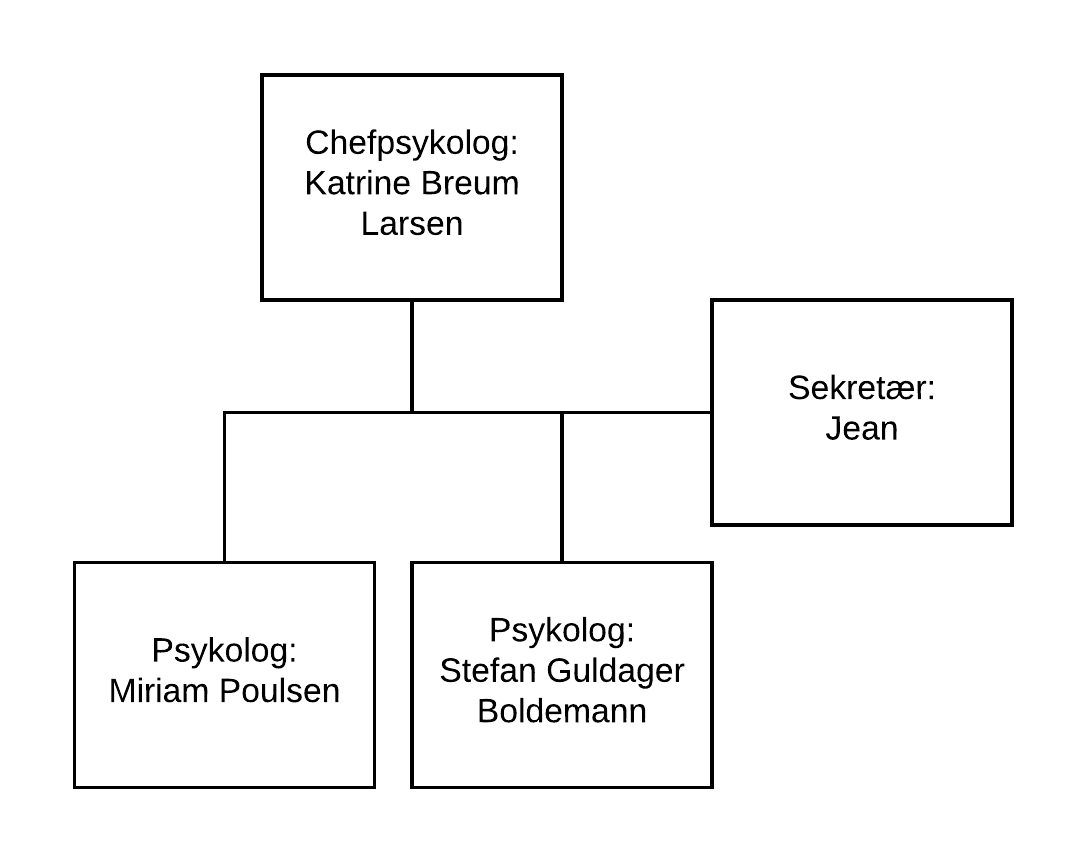
\includegraphics[scale=.8]{OrganisationsDiagram}
    \label{forretning:organisationsdiagram}
\end{figure}

\begin{figure}[ht]
    \caption{FML for PsykologNord}
    \centering
        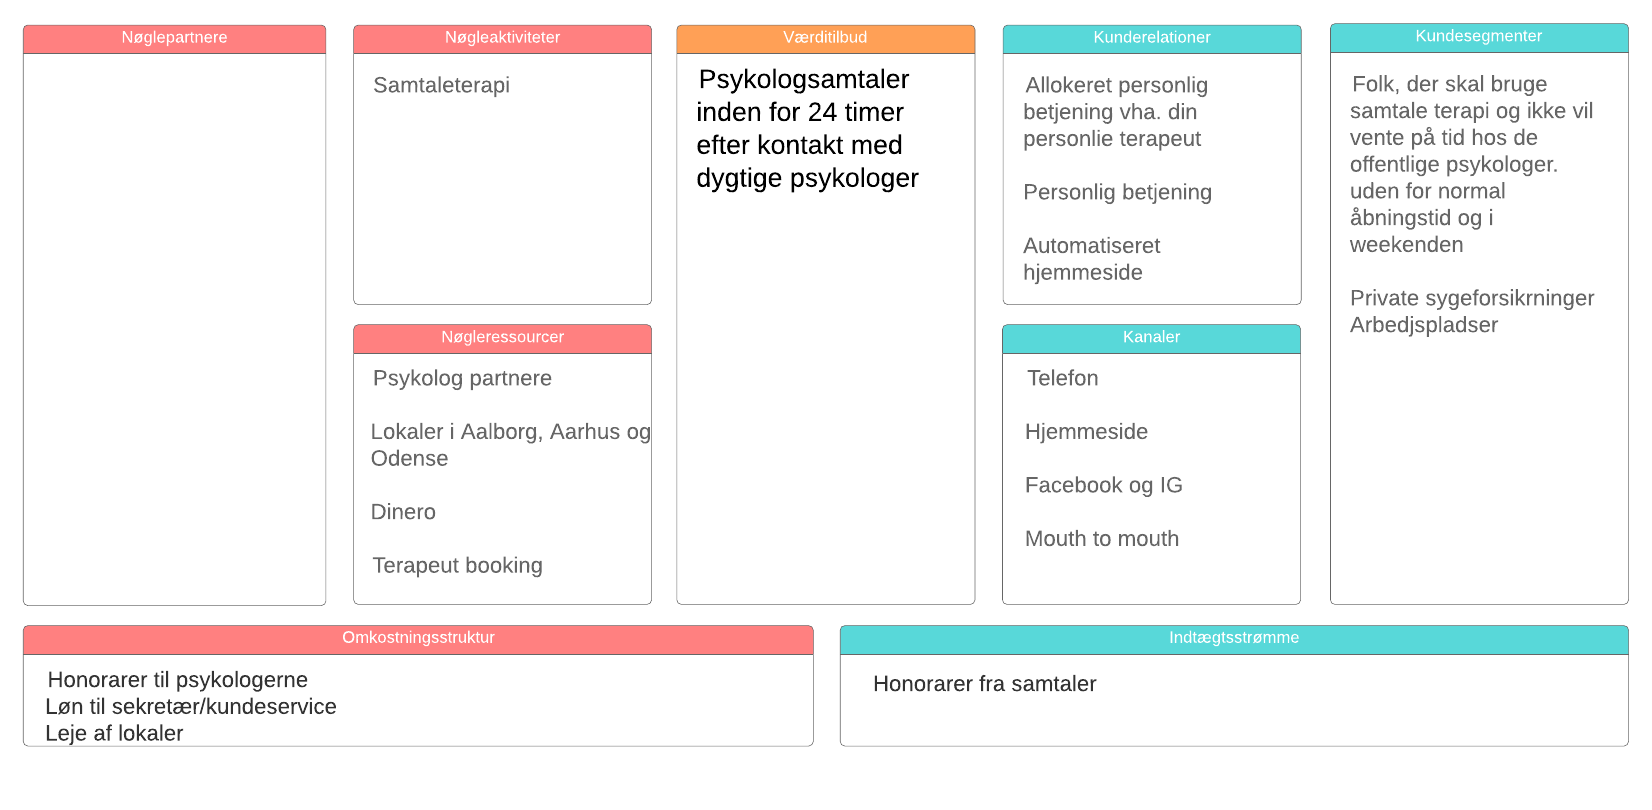
\includegraphics[width=\textwidth]{FML}
    \label{forretning:fml}
\end{figure}

